% Letters
% Letters are short reports of original research focused on an outstanding finding whose importance means that it will be of interest to scientists in other fields.

% They do not normally exceed 4 pages of Nature and, as a guideline, allow up to 30 references. They begin with a fully referenced paragraph, ideally of about 200 words, but certainly no more than 300 words, aimed at readers in other disciplines. This paragraph starts with a 2-3 sentence basic introduction to the field; followed by a one-sentence statement of the main conclusions starting 'Here we show' or equivalent phrase; and finally, 2-3 sentences putting the main findings into general context so it is clear how the results described in the paper have moved the field forwards.

% Please refer to our annotated example to see how the summary paragraph for a Letter should be constructed.

% The rest of the text is typically about 1,500 words long. Any discussion at the end of the text should be as succinct as possible, not repeating previous summary/introduction material, to briefly convey the general relevance of the work.

% Letters typically have 3 or 4 small display items (figures or tables).

% Word counts refer to the text of the paper. References, title, author list and acknowledgements do not have to be included in total word counts.

\documentclass[11pt,letterpaper]{article}

%\usepackage{fontspec}
%\usepackage[utf8]{inputenc}
\usepackage{textcomp,marvosym}
\usepackage{amsmath,amssymb}
\usepackage[normalem]{ulem}
\usepackage[left]{lineno}
\usepackage{booktabs}
\usepackage{changepage}
\usepackage{rotating}
\usepackage{color}
\usepackage{natbib}
\usepackage{setspace}
\usepackage{array}
\usepackage{fancyhdr}
\usepackage{graphicx}
\usepackage{xspace}
\usepackage[hidelinks]{hyperref}
\urlstyle{same}
\usepackage{threeparttable}
\doublespacing

\raggedright
\textwidth = 6.5 in
\textheight = 8.25 in
\oddsidemargin = 0.0 in
\evensidemargin = 0.0 in
\topmargin = 0.0 in
\headheight = 0.0 in
\headsep = 0.5 in
\parskip = 0.1 in
\parindent = 0.2in

% Bold the 'Figure #' in the caption and separate it from the title/caption with a period
% Captions will be left justified
\usepackage[aboveskip=1pt,labelfont=bf,labelsep=period,justification=raggedright,singlelinecheck=off]{caption}

% Remove brackets from numbering in List of References
%\makeatletter
%\renewcommand{\@biblabel}[1]{\quad#1.}
%\makeatother

% Self defined commands
\newcommand{\degreesC}{\textdegree C\xspace}
\newcommand{\degrees}{\textdegree\xspace}
\newcommand{\dC}{$\delta^{13}$C\xspace}
\newcommand{\dO}{$\delta^{18}$O\xspace}
\newcommand{\SrSr}{$^{87}$Sr/$^{86}$Sr\xspace}
\newcommand{\permil}{\textperthousand\xspace}
\newcommand{\dsil}{$d$\xspace}
\newcommand{\UPb}{$^{206}$Pb/$^{238}$U\xspace}
\newcommand{\pCOtwo}{\textit{p}CO$_{2}$\xspace}
\newcommand{\COtwo}{CO$_{2}$\xspace}
%

\pagestyle{myheadings}
\pagestyle{fancy}
\fancyhf{}
\lhead{Park et al., in preparation}
\rhead{\thepage}

\begin{document}

\begin{flushleft}
{\Large \textbf{Growth of the broader Indonesia archipelago as a driver for Neogene cooling}}

Yuem Park\textsuperscript{1},
Nicholas L. Swanson-Hysell\textsuperscript{1},
Pierre Maffre\textsuperscript{1},
Francis A. Macdonald\textsuperscript{2},
Eliel A. Anttila\textsuperscript{2},
Yves Godd\'eris\textsuperscript{3}

\bigskip
\textsuperscript{1} Department of Earth and Planetary Science, University of California, Berkeley, CA, USA

\textsuperscript{2} Department of Earth Science, University of California, Santa Barbara, CA, USA

\textsuperscript{3} G\'eosciences Environnement Toulouse, CNRS--Universit\'e Paul Sabatier - IRD, Toulouse, France

\bigskip

\end{flushleft}

\linenumbers

The broader Indonesia archipelago has an out-sized influence on modern chemical weathering fluxes. The confluence of steep topography, a warm and wet tropical climate, and the presence of mafic lithologies results in high fluxes of Ca and Mg cations and associated \COtwo consumption \citep{Hartmann2009a, Hartmann2014a}. There has been significant growth of land area within the region since the Miocene associated with ongoing arc-continent collision between Australia and the Sunda-Banda arc system (\citealp{Molnar2015a}; Fig. \ref{Fig:indo_growth}). This collision between the Australian-Indian and Eurasian plates and intervening arc terranes has led to the emergence of Indonesia and New Guinea and the exhumation of large supra-subduction ophiolites and associated forearcs in the warm, wet tropics.

Given that the region is a modern-day hot spot of chemical weathering and \COtwo consumption \citep{Hartmann2009a}, what effect has growth of the broader Indonesian archipelago had on Earth's climate state and what would \pCOtwo be on Earth if the region was not there at all? Based on paleogeographic reconstructions of arc-continent collisions through time, \citet{Macdonald2019a} proposed that arc-continent collisions in the tropics are responsible for increasing planetary weatherability, lowering \pCOtwo and causing the onset of glacial climate states. There has been significant planetary cooling since the Mid-Miocene Climatic Optimum leading to the onset of northern hemisphere glaciation, in addition to Antarctic glaciation, over the past few million years \citep{Shackleton1984a}. The \pCOtwo threshold for Antarctic glaciation is estimated to be $\sim$750~ppm with that for northern hemisphere glaciation being significantly lower at $\sim$280~ppm \citep{DeConto2008a} providing an explanation for the delay between southern hemisphere and bipolar glaciation. We seek to evaluate the hypothesis that the growth of the broader Indonesian archipelago has played a significant role in lowering \pCOtwo thereby driving this cooling and the development of northern hemisphere ice sheets.

Over geologic time-scales, \COtwo enters Earth's ocean/atmosphere system primarily via volcanism and metamorphic degassing of the solid Earth, and leaves it primarily through the chemical weathering of silicate rocks, which delivers alkalinity and cations to the ocean that ultimately result in the consumption of carbon via the precipitation of carbonate rocks \citep{Kump2000a}. However, assessing the effect of the growth of the broader Indonesia archipelago on Earth's \pCOtwo levels can not be determined simply through assessing the present-day chemical weathering fluxes. As \COtwo sinks are removed and \COtwo rises, there will be increases in temperature and invigorated hydrological cycling that causes other weathering sinks to increase. The steady-state \pCOtwo of Earth is set by the \pCOtwo level at which the sinks of \COtwo are equal to the sources. The magnitude of the silicate weathering \COtwo sink can be equal to the magnitude of the source at lower \pCOtwo on a planet with relatively high weatherability than on a planet where it is lower \citep{Kump1997a}.

%Imbalances between the magnitude of these source and sink fluxes will cause \pCOtwo to change until the silicate weathering negative feedback (in which elevated \pCOtwo leads to higher temperatures and a more intense hydrological cycle that enhances chemical weathering of silicate rocks and therefore the consumption of \COtwo, and vice versa) stabilizes \pCOtwo at a new steady state value \citep{Walker1981a}. One way to perturb steady state \pCOtwo is to change global weatherability - the sum of factors other than climate that contribute to the chemical weathering of rocks and associated \COtwo consumption, such as lithology \citep{Gaillardet1999a, Dessert2003a}, topography \citep{Maher2014a, Maffre2018a}, and paleolatitude \citep{Swanson-Hysell2017a}. \COtwo input from the solid Earth, assuming that it remains constant, can be removed via silicate weathering at a lower \pCOtwo on a planet with relatively high weatherability than on a planet where it is lower \citep{Kump1997a}.

Topography, climate, and lithology all play important roles in modulating chemical weathering. In low-relief regions, low physical erosion rates lead to a supply-limited weathering regime, in contrast to regions of high denudation where there are higher weathering fluxes \citep{Gabet2009a, West2012a, Maher2014a}. In warm and wet regions, mineral dissolution kinetics are faster leading to enhanced chemical weathering \citep{Lasaga1994a, West2012a}. Regions with high physical weathering rates that are not supply-limited are more sensitive to changes in climate that can enhance the total chemical weathering rate \citep{West2012a, Maher2014a}. In terms of lithology, mafic rocks have the potential to sequester more carbon through silicate weathering because of their relatively high concentrations of Ca and Mg as well as high reaction rates \citep{Dessert2003a}. These factors taken together are what have lead to the proposal that arc-continent collisions within the tropical rain belt have been important in enhancing global weatherability and initiating glacial climate over the past 520~m.y. \citep{Jagoutz2016a, Swanson-Hysell2017a, Macdonald2019a} and perhaps in the Neoproterozoic as well \citep{Park2019a}.

%higher weatherability than felsic rocks because of both the higher concentrations of Ca and Mg (that ultimately sequester carbon through precipitation as carbonate) in mafic lithologies, as well as their faster weathering rates in identical conditions \citep{Dessert2001a, Dessert2003a}. Soil shielding is another important factor that affects weatherability - in low-relief regions, regolith tends to be thicker, which can lead to  In this framework, processes that lead to continued exhumation of mafic lithologies and the creation of steep topography that minimizes soil shielding, particularly in tropical regions where temperature and runoff is high, should exert a strong control on global weatherability and long-term climate. Recent work has suggested that arc-continent collisions in the tropics during the Ordovician \citep{Swanson-Hysell2017a}, the Cenozoic \citep{Jagoutz2016a}, and even the Neoproterozoic \citep{Park2018a} played an important role in initiating glacial climate states at those times. Furthermore, a comparison between the paleolatitudinal position of all major Phanerozoic arc-continent collisions and the latitudinal extent of continental ice sheets reveals a strong correlation between the extent of glaciation and arc-continent collisions in the tropics \citep{Macdonald2019a}. On the other hand, \citet{Park2019a} found no correlation between the extent of glaciation and large igneous province area in the tropics, which was explained by the fact that large igneous provinces, although mafic, are often emplaced into low relief areas where soil shielding is relatively high.

%However, quantifying the increase in global weatherability associated with these tropical arc-continent collisions or large igneous province emplacements and the consequent decrease in steady state \pCOtwo is challenging for the past, primarily due to the large uncertainties on the global context within which these events took place. For instance, in order to even begin to model global weathering fluxes and \pCOtwo, one would need to have constraints on the paleogeographic distribution of land masses, the spatial distribution of temperature, runoff, topography, and lithology on these land masses, and the carbon input flux coming from the degassing of the solid Earth at the time of these events. While the paleogeographic distribution of the continents is broadly well-constrained for recent Earth history (e.g. \citealp{Torsvik2016a}) and temperature and runoff can be estimated using a global climate model, constraints on the other parameters are poor, particularly as we go deeper into Earth's history.

%However, the growth of the Malay Archipelago (the islands of Indonesia and surrounding regions, Fig. X) as Australia migrates northward represents an episode of arc-continent collision occurring in the tropics today. Given that the global context within which this event is occurring is well-constrained, the growth of the Malay Archipelago presents an opportunity to quantify the increase in global weatherability and consequent decrease in steady state \pCOtwo associated with it, and evaluate the feasibility of similar tropical arc-continent collisions initiating glacial climate states throughout Earth's history \citep{Macdonald2019a}.

% \section*{METHODS}

% \subsection*{Paleoshoreline data}

We use geological and paleoshoreline data to quantify the changes in the area of the broader Indonesia archipelago over the past 20~m.y. Following \citet{Molnar2015a}, we analyzed the area changes of islands that are greater than $\sim$200~km, and we also included changes in areas of submerged continental shelves that were previously exposed, like the Sunda Shelf. Carbonate strata and thin-bedded siliciclastic strata were interpreted to represent a subaqueous marine environment, whereas evidence for exposure and terrestrial siliciclastic deposits were used as evidence for a subaerial environment. Taken together, these constraints delineate the position of shorelines. For the island of Sulawesi, we followed the recent stratigraphic compilation and paleoshorelines delineated by \citet{Nugraha2018a} and for New Guinea we followed work of \citet{Norvick2003a, Cloos2005a, Gold2017a}. While there are difference in data sources and paleoshoreline outlines from \cite{Molnar2015a}, the calculated area at 5~Ma is quite similar.

While there has been an increase in land area associated with arc-continent collision, there has also been a decrease in land area associated with subsidence of the Sunda Shelf \citep{Sarr2019a}. Although the majority of the Sunda Shelf is currently submerged, large portions of this low-relief area of continental crust were likely emergent throughout the Neogene, and were repeatedly subaerially exposed during the Pleistocene as recently as the Last Glacial Maximum \citep{Halls2002a}. Similarities in terrestrial biotas of Borneo and mainland Southeast Asia suggest the existence of land bridges on the Sunda Shelf throughout the Miocene \citep{Moss1998a}. During the Eocene through early Miocene, the rifting of the South China Sea resulted in subsidence \citep{Morley2013a} and recent subsidence is interpreted to be a result of dynamic topography, triggered by subduction-related mantle flow \citep{Sarr2019a}. In the Miocene, this region was likely a mixture of crystalline lithologies and siliciclastic sediments similar to eastern Borneo. The relatively low-relief of the region contrasts with the high-relief and mafic lithologies of the broader Indonesia archipelago. We incorporate land area associated with the subsided Sunda Shelf into our modeling.

%From Macdonald text:
%A critical issue for the paleogeographic  analysis of Indonesia is how to deal with the Sunda Shelf. Although the majority of the Sunda Shelf is currently submerged, large portions of this flat-lying, relatively stable platform of continental crust were likely emergent throughout the Neogene, and were repeatedly subaerially exposed during the Pleistocene as recently as the Last Glacial Maximum (38). From a biogeographical standpoint, similarities between the terrestrial biotas of Borneo and mainland Southeast Asia suggest the existence of land bridges on the Sunda Shelf throughout the Miocene (Moss and Wilson, 1998). During the Eocene through early Miocene, the rifting of the South China Sea resulted in subsidence throughout the Sunda Shelf (Morley and Morley, 2013). Grabens associated with this subsidence became freshwater rift lakes that later transitioned to partially-enclosed inland seas and extensive brackish or saline wetland environments. Extensive palynological analysis suggests widespread swamp environments persisting through the Late Miocene (Morley and Morley 2013). Basement highs (e.g. the Natuna Arch, currently subaerially exposed as the largely granitic island of Natuna off SW Borneo, as well as the granitic Tin Islands south of the Malay Peninsula) are typically bounded by Paleogene to Neogene basins dominated by shallow marine clastic fill (Darmadi et al, 2007). Although most paleogeographic reconstructions of the region incorporate some degree of constant exposure of the Sunda Shelf from 20 Ma onwards (Hall, 2013b; Madon et al, 2013), Molnar and Cronin (2015) omit the Sunda Shelf from their paleogeographic model for 5 Ma. We test the sensitivity with two separate scenarios in which the Sunda Shelf is either variably exposed or entirely inundated from 20 Ma to present.

%The areas of Indonesia and New Guinea has substantially increased over this time period with an acceleration over the past 5 million years.

%We then incorporate these rock units into a paleogeographic model to determine the position of these units relative to the warm wet tropics. We find that the subaerially exposed area in the tropics of Indonesia and New Guinea has steadily increased through the Neogene with an acceleration over the past 5 Myrs.

% \subsection*{GEOCLIM}

To estimate the decrease in steady state \pCOtwo associated with the increase in global weatherability from the growth of the broader Indonesia Archipelago, we use the spatially resolved GEOCLIM model \citep{Godderis2014a, Godderis2017c} wherein a silicate weathering model is coupled to climate models run at varying \pCOtwo levels. We use the DynSoil implementation of the \cite{Gabet2009a} regolith development model which integrates a climatic dependence on the chemical weathering using the formulation of \cite{West2012a}. Changes in silicate weathering lead to changes in \pCOtwo with the climate models being used to estimate temperature and runoff fields which then modulates the silicate weathering

then iteratively

%which iteratively couples box models of surface biogeochemical cycles to climate model output. Estimates of fluxes of species between carbon, alkalinity, phosphorous, and oxygen reservoirs in the ocean and atmosphere are used to calculate \pCOtwo, which is then compared against climate model output computed at various \pCOtwo levels to estimate temperature and runoff at the current \pCOtwo in GEOCLIM. These new temperature and runoff fields are then fed back into the biogeochemical box models to update \pCOtwo, for which new temperature and runoff fields are again estimated. This iteration is continued until a steady state is achieved in all reservoirs.

In this study, we use temperature and runoff fields from a subset of the GFDL CM2.0 experiments \citep{Delworth2006a, Delworth2006b} for the climate model component of GEOCLIM. These experiments were performed in order to explore the effect of various changes in forcing agents on climate since ca. 1860 at a 1\degrees $\times$ 1\degrees resolution. In the `1860 control' experiment, forcing agents representative of conditions ca. 1860 (including \COtwo, CH$_{4}$, N$_{2}$O, O$_{3}$, sulfates, carbon, dust, sea salt, solar irradiance, and the distribution of land cover types) are held constant for 500 years after reaching equilibrium. \pCOtwo in 1860 is assumed to be 286~ppm. In the `+1\%/yr to 2$\times$' experiment, initial conditions are taken from the `1860 control' experiment, then \pCOtwo is prescribed to increase from 286~ppm at a compounded rate of +1\% per year for 70 years, when \pCOtwo reaches double (572~ppm) of the initial value. \pCOtwo is then held constant until the end of the 280 year experiment. All non-\COtwo forcing agents are held constant. The `+1\%/yr to 4$\times$' experiment is identical to the `+1\%/yr to 2$\times$' experiment, except that \pCOtwo is prescribed to increase for 140 years, when \pCOtwo reaches quadruple (1144~ppm) of the initial value. We take the mean of the last 100 years of each of these three experiments (when \pCOtwo is being held constant at its final level) to obtain temperature and runoff fields for 286, 572, and 1144~ppm respectively. The primary strength of using these three GFDL CM2.0 experiments is that all non-\COtwo forcing agents are held constant, allowing the effect of \pCOtwo on climate to be isolated.

The silicate weathering component of GEOCLIM calculates \COtwo consumption by silicate weathering for each continental grid cell. In previous versions of the model, the silicate weathering rate was a function of temperature and runoff only, and assumed that the bedrock in all continental grid cells had identical chemical compositions (e.g. \citealp{Godderis2014a}). However, more recent versions of GEOCLIM implement regolith development and soil shielding into the silicate weathering component based on work by \citet{Heimsath1997a}, \citet{Gabet2009a}, \citet{West2012a}, \citet{Carretier2014a}, \citet{Godderis2017b}, and \citet{Maffre2018a}, which introduces an additional dependence on topographic slope (see Data Repository). While this introduction of regolith development into GEOCLIM is an important piece of assessing the impact of arc-continent collisions in the Malay Archipelago on \pCOtwo, the relatively high Ca and Mg concentration in arc rocks relative to other lithologies must also be considered. We therefore implement variable bedrock Ca+Mg concentration into the silicate weathering component of GEOCLIM. The spatial distribution of lithologies is sourced from the global lithologic map (GLiM) of \citet{Hartmann2012a}. 16 lithologic categories are represented in GLiM, which we simplify into 6 broader categories: metamorphic, felsic, intermediate, mafic, carbonate, and siliciclastic sediment (Fig. XX; see Data Repository). Each continental grid cell is then assigned one of these lithologic categories. The Ca+Mg concentrations of felsic, intermediate, and mafic grid cells are then assigned based on the mean of MgO and CaO measurements on rocks of each of these lithologic categories in the EarthChem Portal (\url{www.earthchem.org/portal}). The weathering of carbonate grid cells does not contribute to long-term \COtwo consumption and therefore its Ca+Mg concentration is ignored. The Ca+Mg concentrations of metamorphic and siliciclastic sediment grid cells are more difficult to define, since the chemical composition of these two lithologic classes is strongly dependent on its protolith. The chemical composition of siliciclastic sediment is further strongly dependent on its degree of chemical depletion. We therefore explore a range of feasible Ca+Mg concentrations of metamorphic and siliciclastic sediment grid cells during the calibration of the silicate weathering component of GEOCLIM (see below).

\subsection*{Parameter Calibration}

The silicate weathering component of GEOCLIM models the geochemical evolution of a rock particle as it leaves unweathered bedrock and transits through overlying regolith (see Data Repository). As the rock particle transits through the regolith, some fraction of the weatherable phases in the rock particle are dissolved and leaves the regolith column as weathered phases. The fraction of the weatherable phases in the rock particle that are not dissolved after transiting through the regolith column leaves it via erosion. Central to this model is the dissolution rate constant, which describes the rate at which weatherable phases in the rock particle are dissolved as it transits through the regolith:

\begin{equation}
    k_{d}\left(1-e^{-k_{w}q}\right)e^{-\frac{E_{a}}{R}\left(\frac{1}{T}-\frac{1}{T_{0}}\right)}\tau^{\sigma}
    \label{eq:1}
\end{equation}

$q$ is the runoff, $E_{a}$ is the activation energy, $R$ is the universal gas constant, $T$ is the temperature, $\tau$ is the time that a given rock particle has spent in the regolith, and $k_{d}$, $k_{w}$, and $\sigma$ are calibration constants.



clean up equation - add units?

allbcc vs lith map

XXX


\begin{itemize}
    \item GEOCLIM and GFDL models
    \item added lithology (GLiM)
    \item calibration
    \item tested scenarios
    \item in discussion, talk about GFDL limitations (equilibrated by last 100 years?, not changing paleogeography, low resolution, model is quite old)
\end{itemize}

The global lithological map database GLiM of Hartmann and Moosdorf was used to develop a

The lithological categories of the global lithological map database GLiM of \cite{Hartmann2012a} were used and grouped into 6 categories: metamorphic, felsic, intermediate, mafic, carbonate, and siliciclastic. These values were assigned at the 0.5\textdegree resolution and were then downsampled using a mode downsampling scheme to 1\textdegree resolution

\section*{RESULTS}

XXX

\section*{DISCUSSION}

After the Miocene Climatic Optimum, a cooling trend began ca. 15 Ma that accelerated over the past 5 Ma. Many hypotheses have been proposed to explain this cooling trend.... One of these hypotheses is that

Discuss source term. Can cite: https://doi.org/10.1093/gji/ggw277 related to spreading rate.

\section*{ACKNOWLEDGEMENTS \label{sec:ACKNOWLEDGEMENTS}}

XXX

\clearpage
\newpage

\section*{TABLES}

XXX

\clearpage
\newpage

\section*{FIGURES}

\begin{figure}
    \centering
    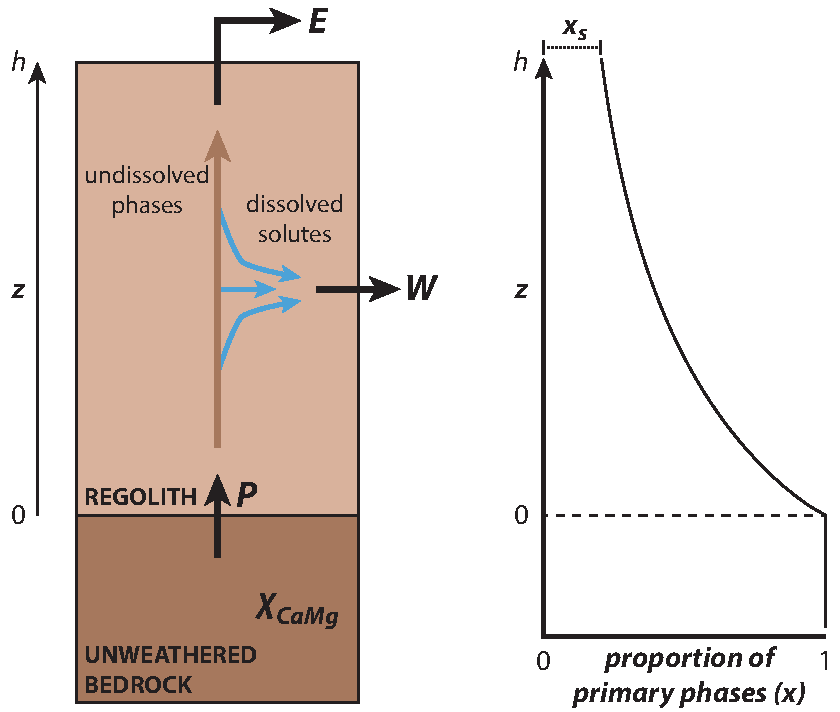
\includegraphics{Manuscript/Figures/regolith_schematic.pdf}
    \caption{Growth of the broader Indonesia archipelago. Past shorelines are shown in A with resultant area estimates summarized in B. A significant increase in area over the past 5 million years is coincident with cooling and the onset of Northern Hemisphere glaciation as reflected in the benthic oxygen isotope record in C \cite{Zachos2008a}.}
    \label{fig:my_label}
\end{figure}

\clearpage
\newpage
\footnotesize

\singlespacing

\bibliographystyle{gsabull}
\bibliography{References}

\end{document}

Text from Francis draft on shoreline analysis:

Neogene cooling and the emergence of Indonesia and New Guinea

Abstract
The cooling trend from 15 Ma to present coincides with arc-continent collision and exhumation in Indonesia and New Guinea. To assess relationships between the emergence of highly weatherable arc terranes with tectonic topography in the tropics, an increase in global weatherability, geochemical records, and climate change, we use geological and paleoshoreline data quantify the changes in the area of volcanic and ultramafic rocks in Indonesia and New Guinea over the past 20 Myrs. We then incorporate these rock units into a paleogeographic model to determine the position of these units relative to the warm wet tropics. We find that the subaerially exposed area in the tropics of Indonesia and New Guinea has steadily increased through the Neogene with an acceleration over the past 5 Myrs. Arc-continent collision has resulted in the exhumation of both the East Sulawesi and Irian Jaya-New Guinea ophiolites, which are two of the three largest preserved ophiolites on Earth. We suggest that cooling from 15 to 10 Ma was due in large part to the subaerial exposure of these ophiolites and increase in global weatherability, and that the more recent acceleration in cooling was due to increased exhumation rates in Indonesia and New Guinea. Both a decrease of mid ocean ridge spreading rates and changes in the composition and amount of riverine input is necessary to explain both global cooling and geochemical proxy data. The data presented herein helps disentangle these effects.

Significance statement
	The tectonic drivers for the Neogene cooling trend from ~15 Ma to present are unknown. Here we quantify paleoshoreline data in Indonesia and New Guinea over the Neogene to assess the hypothesis that cooling was caused by changes in paleogeography in the warm wet tropics. These data document the emergence of Indonesia over this interval and are consistent with changes in global weatherability associated with arc-continent collision in the  tropics as a major driver of long-term climate change.

\body
After the Miocene Climatic Optimum (MCO), a cooling trend began at ~15 Ma, and accelerated over the past 5 Ma (1-4) (Fig. 1).  Many hypotheses have been proposed to explain this cooling trend including changes in ocean circulation and upwelling (5, 6), perhaps associated with increased organic carbon burial (7, 8) or the closure of the  Central American Seaway (9), an increase in the strength of the Walker Circulation associated with the growth of Indonesia (10), feedbacks with terrestrial vegetation (11), a decrease in volcanic outgassing (12), an increase in basaltic watersheds in the tropics (10, 13), uplift in the Himalayas (14), and arc-continent collision in the tropics (15). Although changes in circulation and vegetation may have contributed to these signals on hundreds of thousands to million year timescales, the global extent and multi-million year timescale suggests that the long-term cooling trend since 15 Ma is the product of changes in the geological sources and sinks of carbon, modulated by the silicate weathering feedback (16-20).
On geological timescales, atmospheric CO2 levels can vary due to changes in volcanic CO2 flux, but also due to changes in global weatherability — the cumulative factors that affect chemical weathering aside from climate (20, 21). Global weatherability is the product of variables such as lithology, tectonic uplift rates, and paleolatitude (20). An increase in global weatherability can result in cooling as the consumption of carbon through silicate weathering will match that of volcanic input at lower concentrations of atmospheric CO2 (20).
Present-day global CO2-consumption estimates emphasize the importance of highly weatherable areas: ~10-20% of land area is responsible for ~50-75% of CO2 consumption through silicate weathering and associated carbonate precipitation (22, 23). These highly weatherable areas (e.g. Indonesia and New Guinea) are mainly situated in the warm, wet tropics with significant topographic relief, and have bedrock composed of Ca- and Mg-rich mafic and ultramafic lithologies, which have faster dissolution rates than felsic rocks (20, 23, 24). As a result of the intertropical convergence zone (ITCZ), and its migration through the year, annual rainfall on Earth is greatest within ~15º of the equator resulting in the tropical rain belt. Given that hemispherically asymmetric forcings are relatively small, the position of the ITCZ is interpreted to be stable even with large changes in forcing resulting from changing CO2 levels (25). In modern climate data, the region within 10º of either side of the equator corresponds with precipitation greater than 1.5 m/yr and the region within 15º corresponds with precipitation greater than 1.0 m/yr. Because of the strong relationship between runoff and silicate weathering (26), paleogeographic changes in tropics, particularly in tropical regions with tectonic topography and abundant volcanic rocks, like Indonesia and New Guinea, should have an outsized effect on the Earth’s long-term climate state (10, 15).
Recently, it was proposed that arc-continent collision in the tropics drove the cooling trend over the past 15 million years (15, 27). This hypothesis builds off of the suggestion of Reusch and Maasch (28) that arc-continent collisions could accomplish both a decrease in outgassing by terminating arc volcanism (footnote: However, arc-continent collision generally results in subduction flip with renewal of arc magmatism (29)), and an increase in silicate weathering by exhuming soluble Ca- and Mg-rich silicate rocks. Jagoutz et al. (27) applied this process specifically to the closure of the Neo-Tethys ocean in the tropics and suggested that arc-continent collisions at approximately 80 and 50 Ma could account for the long-term, two-phased cooling trend from the Cretaceous to the E-O boundary. Importantly, Jagoutz et al. (27) combined the Himalayan uplift hypothesis (14) with the basalt drift hypothesis (13, 30), emphasizing that topography, precipitation in the tropical rain belt, and lithology are the key variables in global weatherability. Macdonald et al. (15) compiled paleolatitude data on ophiolite bearing sutures through the Phanerozoic and concluded that the extent of arc-continent collisions tropics correlates with extent of continental glaciation, and specifically, that arc-continent collisions in Indonesia and New Guinea were associated with cooling over the past 15 Myr.
Due to rugged tectonic topography (Fig. 2A), tropical temperatures and precipitation rates (Fig. 2B), and a predominance of highly soluble mafic and ultramafic rocks (Fig. 3A), watersheds in Indonesia and New Guinea have the highest rates of silicate weathering in the world accounting for ~9% of the modern global carbon sink (23, 26). Although there are significant monsoonal and orographic effects in Indonesia, and particularly in New Guinea (Fig. 2A), the high mean annual rainfall sill results in rivers with the highest average silicate weathering rates (26). Recognizing the importance of the paleogeography of this region, Molnar and Cronin (10) used paleoshoreline data to estimate that the area of subaerially exposed landmass in Indonesia and New Guinea increased by 60% over the last 5 Myrs. Here we quantify the changes in exposed area and rock types in the tropical region of Indonesia and New Guinea over the past 20 Myrs in a paleogeographic model. These results allow us to assess the changes of mafic and ultramafic rocks in the warm wet tropics of Indonesia and New Guinea throughout the Neogene and test the hypothesis that the subaerial emergence of this region associated with arc-continent collision caused an increase in global weatherability and cooling. These data can further be incorporated into future coupled climate and weathering models to assess the effect of changing paleogeography and global weatherabilty on long-term climate state.

Tectonic Evolution
During Neogene arc-continent collision between the Australian-Indian and Eurasian plates and intervening arc terranes (31-33), Indonesia and New Guinea emerged as several large supra-subduction ophiolites and associated forearcs were exhumed in the warm, wet tropics. Some of these ophiolites formed immediately prior to collision and others have an older history.
The oldest ophiolites preserved in the Indonesia orogenic system are situated in the northwest and associated with the easternmost Paleo-Tethyan sutures (34). On the Malay Peninsula, the Bentong-Raub belt (suture 1; Fig. 3) demarcates the eastern margin of Cimmerian ribbon continent Sibumasu, which collided with the Suhothai arc in the latest Permian to early Triassic (34). Thermochronology suggests that the  Malay Peninsula was first exhumed during the mid-Eocene to early Oligocene (35). This region became a significant sediment source for the Crocker Fan on the NW margin of Borneo during the Oligocene (36), as well as to the east of Malay Peninsula during the Neogene, and has been largely exposed over the last 20 Ma (37, 38).
In Sumatra, the Wolya arc (suture 2; Fig. 3) formed at 95 Ma and is overlain by Campanian 83.5-70.6 Ma radiolarian cherts (39), which were uplifted and eroded from 60-40 Ma (40). These ophiolites were entrained in the Banda Arc, which has experienced magmatism and accretion throughout most of the Cenozoic as the Australian plate subducts beneath it (37, 41). From ~20-10 Ma, the majority of Sumatra was submerged, although Bangka and Belitung were exposed in addition to a portion of the greater Sunda Shelf, which was at least partially exposed throughout the past 20 Ma (37, 41). Most of Sumatra was submerged until after 5 Ma with the arrival of the leading edge of continental Australia (37, 41).
The Meratus belt (sutures 3 and 4; Fig. 3), which extends from Java (42) through eastern Borneo (43) to Palawan (44), marks the Late Cretaceous collision of the Banda blocks and Argo. After this collision, subduction polarity reversed and a Cretaceous to Miocene SE-facing volcanic arc developed (45), which we refer to here as the Great Indonesian arc. In southern Borneo, sedimentological data in the adjacent Barito Basin suggests that ophiolites in the Meratus Mountains were not emergent until the Late Miocene (46). In northern Borneo and Palawan, collision occurred in the Late Oligocene to Early Miocene, resulting in exhumation of the Palawan Ophiolite Complex (44, 46). Over 10 km of Neogene sediment fills the Sarawak Basin and NW Borneo trough, indicative of extensive exhumation and erosion in northern Borneo (36). Thermochronological data suggest extremely rapid uplift (7 km/Myr) and exhumation during the Late Miocene and Early Pliocene, resulting in the recent formation of Mt. Kinabalu, the tallest peak in Borneo (47).
The East Sulawesi ophiolite (suture 5; Fig. 3) was likely generated in a supra-subduction to backarc setting in the Great Indonesian arc (45, 48, 49) [but see (50) for an alternative view], detached from its metamorphic sole in the late Oligocene (32-28 Ma; 51), and subsequently thrust to the east above a west dipping slab. During the Early to Middle Miocene, the Tukang Besi-Buton block began to collide obliquely with the southeastern end of the Sunda Arc, causing additional ophiolite emplacement in west and southeast Sulawesi, including Buton (52, 53). Uplift was diachronous, not effecting units is western Sulawesi until the Middle Miocene (~13 Ma) (54). Exhumation is recorded by the presence of a major Middle Miocene unconformity and sedimentary breccias in marginal basins (52, 54). Collision of the Sula-Banggai block with the east margin of Sulawesi began in the Late Miocene and uplift accelerated in the Early Pliocene (5.2 to 3.8 Ma) and is associated with a major pulse of sedimentation in adjacent basins (55, 56). Off the northeastern margin of the east arm of Sulawesi, Miocene platform carbonates on the Sula-Banggai block are overlain by Late Miocene to Early Pliocene ophiolite detritus in the Celebes mélange (55). Thus, although the East Sulawesi ophiolite was trapped/emplaced onto the composite Sundaland margin (i.e. a fragment of previously accreted Australian crust) between 36 and 23 Ma, mafic and ultramafic rocks appear to have not been substantially subaerially exposed in the south and west arms until after 15 Ma, and on the east arm until after 5 Ma. Thermochronology indicates that exhumation accelerated in the Late Miocene to Pliocene (52-54, 57). North Sulawesi, where active volcanoes extend through the Sangihe Arc into the southern Philippines, was not substantially emergent until the Pliocene (58).
Along the Papuan Peninsula of Eastern New Guinea, Oligocene arc-continent collision between Australian continental fragments and the Inner Melanesian arc exhumed the Papuan Ultramafic Belt (Fig. 3; suture 6) above a north dipping slab (59, 60). In the Central Range of New Guinea, a second set of arc-continent collisions in New Guinea began in the Middle Miocene with the collision between the Outer Melanesian arc and the distal margin of Australia (59, 61, 62). This resulted in the exhumation of the 1440 km long Irian-Marum-April ophiolite belt (Fig. 3; suture 7). The Middle Miocene (16–14 Ma) basal Markats Formation contains siliciclastic sediment that was transported from the south into the forearc basin associated with the PNG ophiolite belt (61, 63). This precedes, by several million years, the beginning of widespread synorogenic sedimentation to the south and on the Australian continental basement at ca. 12 Ma (59). Mountain building began in the Late Miocene, ca. 8-7 Ma (59, 62) with 3-4 km of denudation between 8-5 Ma (64), but major relief was not generated until the Pliocene (65). Exhumation of the Central Range accelerated over the past 5 Myrs due to slab-breakoff and buoyant uplift under New Guinea (61). Although the Papuan Ultramafic Belt was generated and obducted earlier than the ophiolites in the Central Range (60, 66), it was also exhumed very rapidly over the past 10 Ma (62).
After arc-continent collision in New Guinea, a left-lateral strike-slip margin developed on the northern margin (62). Over the past 4 Myr, this change in plate motion caused the westward extrusion and exhumation of the Cretaceous to Oligocene ophiolites of Obi (67), Halmahera (68, 69), and northern New Guinea (70) (Fig. 3; sutures 8-10). In the Bird’s Head region, this change in plate motion led to CCW rotation and the exhumation of several core complexes (71).
The Philippine ophiolites have been grouped in four distinct belts (72). We combine belts 1 and 2 in an eastern suture zone and belts 3 and 4 in a western suture zone (Fig. 3; sutures 11 and 12). Belts 1 and 2 were juxtaposed in the eastern suture zone during sinistral transpression, which resulted in Early Miocene uplift and deposition of coarse clastic sediments (73). The Palawan microcontinental block and Philippine mobile belt collided during late Early Miocene to early Middle Miocene resulting into the emplacement of the western ophiolites, with exhumation extending from the Late Miocene to the present (74).
In addition to collision, arc magmatism may have contributed more significantly to crustal growth in the Philippines (75).
The youngest ophiolites of Indonesia formed in the Banda Sea starting at ca. 15 Ma (33). The ongoing arc-continent collision became emergent in Seram and Timor (Fig. 3; sutures 13 and 14) over the last 5 Myr, as the Banda arc began to abut the Banda embayment emplacing the Timor nappe (49, 76, 77).

Paleoshorelines
Geological maps and paleoshoreline data were used to calculate the changes in different types of subaerially exposed rocks in Indonesia and New Guinea. Following Molnar and Cronin (10), we analyzed the area changes of islands that are greater than ~200 km, and we also included changes in areas of submerged continental shelves that were previously exposed, like the Sunda shelf. Larger islands were further divided into regions based upon their position on microplates as defined by Matthews, et al. (78). Lithological maps were modified from Hartmann and Moosdorf (79) and then supplemented with regional geological maps. From these maps, the percentage of ultramafic and volcanic rocks relative to other rock types was calculated in QGIS for each island and microplate region.
Generally, the paleoshoreline reconstructions within the paleogeographic models coincide with sub-Epoch boundaries, i.e. Early Miocene = 23-16 Ma, Middle Miocene = 15.99-11.61 Ma, Late Miocene = 11.6-5.4 Ma, Pliocene =5.39-3.8 Ma. However, some additional shorelines have been added where additional age information is present to refine the timing of major changes in area. Miocene to present stratigraphic columns were compiled from each region to develop an age model for various paleoenvironmental indicators. In general, carbonate strata and thin-bedded siliciclastic strata were assumed to be deposited in a subaqueous marine environment, whereas evidence for exposure and terrestrial siliciclastic deposits were used as evidence for subaerial environment. Following previous work on paleoshorelines and these environmental indicators, paleoshorelines were outlined in QGIS to calculate areas for the Early Pliocene (5 Ma), Late Miocene (10 Ma), Middle Miocene (15 Ma), and Early Miocene (20 Ma).
We used geological maps and paleoshoreline data to calculate the changes in different types of subaerially exposed rocks in Indonesia and New Guinea. Using Gplates, paleoshoreline shapefiles were incorporated in the paleogeographic model of Matthews, et al. (78). Although there are some differences between this reconstruction and the recent reconstruction of Hall (33), these do not entail significant changes in paleolatitude.
Many new sources for paleoshoreline data have become available since Molnar & Cronin (10). Particularly, for Sulawesi, we followed the recent stratigraphic compilation and paleoshorelines delineated by Nugraha and Hall (80), and in New Guinea, we followed Gold et al. (81),  Cloos et al. (61), Norvick (2003) and derivative work by Harrington et al. (82), and Nichols and Hall (1991). We also compiled our own stratigraphies for the region to provide further paleoenvironmental context. Although the outlines of our paleoshorelines are very different from those of Molnar & Cronin (10) our calculated area for 5 Ma is not substantially different (Fig. X).
A critical issue for the paleogeographic  analysis of Indonesia is how to deal with the Sunda Shelf. Although the majority of the Sunda Shelf is currently submerged, large portions of this flat-lying, relatively stable platform of continental crust were likely emergent throughout the Neogene, and were repeatedly subaerially exposed during the Pleistocene as recently as the Last Glacial Maximum (38). From a biogeographical standpoint, similarities between the terrestrial biotas of Borneo and mainland Southeast Asia suggest the existence of land bridges on the Sunda Shelf throughout the Miocene (Moss and Wilson, 1998). During the Eocene through early Miocene, the rifting of the South China Sea resulted in subsidence throughout the Sunda Shelf (Morley and Morley, 2013). Grabens associated with this subsidence became freshwater rift lakes that later transitioned to partially-enclosed inland seas and extensive brackish or saline wetland environments. Extensive palynological analysis suggests widespread swamp environments persisting through the Late Miocene (Morley and Morley 2013). Basement highs (e.g. the Natuna Arch, currently subaerially exposed as the largely granitic island of Natuna off SW Borneo, as well as the granitic Tin Islands south of the Malay Peninsula) are typically bounded by Paleogene to Neogene basins dominated by shallow marine clastic fill (Darmadi et al, 2007). Although most paleogeographic reconstructions of the region incorporate some degree of constant exposure of the Sunda Shelf from 20 Ma onwards (Hall, 2013b; Madon et al, 2013), Molnar and Cronin (2015) omit the Sunda Shelf from their paleogeographic model for 5 Ma. We test the sensitivity with two separate scenarios in which the Sunda Shelf is either variably exposed or entirely inundated from 20 Ma to present.
Independent of the Sunda Shelf, our studies suggest that the volume of sediment eroded from Indonesia and New Guinea has exponentially increased over the past 15 Ma, particularly in New Guinea.DISCUSS CHANGES FOR EACH REGION.

References
1.	Zachos J, Pagani M, Sloan L, Thomas E, & Billups K (2001) Trends, Rhythms, and Aberrations in the Global Climate 65 Ma to present. Science 292:686-693.
2.	Cramer B, Miller K, Barrett P, & Wright J (2011) Late Cretaceous–Neogene trends in deep ocean temperature and continental ice volume: Reconciling records of benthic foraminiferal geochemistry (δ18O and Mg/Ca) with sea level history. Journal of Geophysical Research: Oceans 116(C12).
3.	Herbert TD, et al. (2016) Late Miocene global cooling and the rise of modern ecosystems. Nature Geoscience 9(11):843-847.
4.	Zachos JC, Dickens GR, & Zeebe REJN (2008) An early Cenozoic perspective on greenhouse warming and carbon-cycle dynamics. 451(7176):279.
5.	Shevenell AE, Kennett JP, & Lea DW (2004) Middle Miocene southern ocean cooling and Antarctic cryosphere expansion. Science 305(5691):1766-1770.
6.	Holbourn A, Kuhnt W, Kochhann KG, Andersen N, & Sebastian Meier KJG (2015) Global perturbation of the carbon cycle at the onset of the Miocene Climatic Optimum. 43(2):123-126.
7.	Vincent E & Berger W (1985) Carbon dioxide and polar cooling in the Miocene: The Monterey hypothesis. AGU Geophysical Mongograph Series. The Carbon Cycle and Atmospheric CO2: Natural Variations from Archean to Present 32:455-468.
8.	Flower BP & Kennett JPJG (1993) Relations between Monterey Formation deposition and middle Miocene global cooling: Naples Beach section, California. 21(10):877-880.
9.	Haug GH & Tiedemann RJN (1998) Effect of the formation of the Isthmus of Panama on Atlantic Ocean thermohaline circulation. 393(6686):673.
10.	Molnar P & Cronin TW (2015) Growth of the Maritime Continent and its possible contribution to recurring Ice Ages. Paleoceanography 30(3):196-225.
11.	Cerling TE, et al. (1997) Global vegetation change through the Miocene/Pliocene boundary. Nature 389(6647):153-158.
12.	Berner RA, Lasaga AC, & Garrels RM (1983) The carbonate-silicate geochemical cycle and its effect on atmospheric carbon dioxide over the past 100 million years. American Journal of Science 283:641-683.
13.	Kent DV & Muttoni G (2013) Modulation of Late Cretaceous and Cenozoic climate by variable drawdown of atmospheric pCO2 from weathering of basaltic provinces on continents drifting through the equatorial humid belt. Climate of the Past 9(2):525.
14.	Raymo ME, Ruddiman WF, & Froelich PN (1988) Influence of late Cenozoic mountain building on ocean geochemical cycles. Geology 16(7):649-653.
15.	Macdonald FA, Swanson-Hysell NL, Park Y, & Lissiecki LE (2019) Arc-continent collisions in the tropics set the Earth’s climate state. Science 364:181-184.
16.	Walker JCG, Hays PB, & Kasting JF (1981) A negative feedback mechanism for the long-term stabilization of the earth's surface temperature. Geophysical Research Letters 86:9776-9782.
17.	Raymo ME (1991) Geochemical evidence supporting TC Chamberlin's theory of glaciation. Geology 19(4):344-347.
18.	Berner RA (1994) Geocarb II: a revised model of atmospheric CO2 over Phanerozoic time. American Journal of Science 294:56-91.
19.	Berner RA & Caldeira K (1997) The need for mass balance and feedback in the geochemical carbon cycle. Geology 25(10):955-956.
20.	Kump LR & Arthur MA (1997) Global chemical erosion during the Cenozoic: Weatherability balances the budgets. Tectonic Uplift and Climate Change,  (Springer), pp 399-426.
21.	Maher K & Chamberlain C (2014) Hydrologic regulation of chemical weathering and the geologic carbon cycle. Science 343(6178):1502-1504.
22.	Hartmann J, Moosdorf N, Lauerwald R, Hinderer M, & West AJ (2014) Global chemical weathering and associated P-release—The role of lithology, temperature and soil properties. Chemical geology 363:145-163.
23.	Dessert C, Dupré B, Gaillardet J, François LM, & Allegre CJ (2003) Basalt weathering laws and the impact of basalt weathering on the global carbon cycle. Chemical Geology 202(3):257-273.
24.	Ibarra DE, et al. (2016) Differential weathering of basaltic and granitic catchments from concentration–discharge relationships. 190:265-293.
25.	Donohoe A, Voigt AJCEP, & Mechanisms (2017) Why Future Shifts in Tropical Precipitation Will Likely Be Small: The Location of the Tropical Rain Belt and the Hemispheric Contrast of Energy Input to the Atmosphere.115-137.
26.	Gaillardet J, Dupré B, Louvat P, & Allegre C (1999) Global silicate weathering and CO 2 consumption rates deduced from the chemistry of large rivers. Chemical geology 159(1):3-30.
27.	Jagoutz O, Macdonald FA, & Royden L (2016) Low-latitude arc–continent collision as a driver for global cooling. Proceedings of the National Academy of Sciences 113(18):4935-4940.
28.	Reusch DN & Maasch KA (1998) The transition from arc volcanism to exhumation, weathering of young Ca, Mg, Sr silicates, and CO2 drawdown. Oxford Monographs on Geology and Geophysics 39:261-276.
29.	McKenzie DP (1969) Speculations on the consequences and causes of plate motions. Geophysical Journal International 18(1):1-32.
30.	Kent DV & Muttoni G (2008) Equatorial convergence of India and early Cenozoic climate trends. Proceedings of the National Academy of Sciences 105(42):16065-16070.
31.	Hall R (1996) Reconstructing Cenozoic SE Asia. Geological Society, London, Special Publications 106(1):153-184.
32.	Hamilton WB (1979) Tectonics of the Indonesian region (US Govt. Print. Off.).
33.	Hall R (2017) Southeast Asia: New Views of the Geology of the Malay Archipelago. Annual Review of Earth and Planetary Sciences 45(1).
34.	Metcalfe I (2013) Gondwana dispersion and Asian accretion: tectonic and palaeogeographic evolution of eastern Tethys. Journal of Asian Earth Sciences 66:1-33.
35.	Cottam MA, Hall R, & Ghani AAJJoAES (2013) Late Cretaceous and Cenozoic tectonics of the Malay Peninsula constrained by thermochronology. 76:241-257.
36.	Hall R, van Hattum MW, & Spakman WJT (2008) Impact of India–Asia collision on SE Asia: the record in Borneo. 451(1-4):366-389.
37.	Hall R (2013) The palaeogeography of Sundaland and Wallacea since the Late Jurassic. Journal of Limnology 72(s2):1.
38.	Hall R & Nichols GJGS, London, Special Publications (2002) Cenozoic sedimentation and tectonics in Borneo: climatic influences on orogenesis. 191(1):5-22.
39.	Pedersen R, Searle M, Carter A, & Bandopadhyay P (2010) U–Pb zircon age of the Andaman ophiolite: implications for the beginning of subduction beneath the Andaman–Sumatra arc. Journal of the Geological Society 167(6):1105-1112.
40.	Allen R, et al. (2008) New constraints on the sedimentation and uplift history of the Andaman-Nicobar accretionary prism, South Andaman Island. 436:223.
41.	Hall R (2009) The Eurasian SE Asian margin as a modern example of an accretionary orogen. Geological Society, London, Special Publications 318(1):351-372.
42.	Wakita K (2000) Cretaceous accretionary–collision complexes in central Indonesia. Journal of Asian Earth Sciences 18(6):739-749.
43.	Monnier C, et al. (1999) Extensional to compressive Mesozoic magmatism at the SE Eurasia margin as recorded from the Meratus ophiolite (SE Borneo, Indonesia). Geodinamica Acta 12(1):43-55.
44.	Yumul Jr GP, Dimalanta CB, Marquez EJ, & Queaño KL (2009) Onland signatures of the Palawan microcontinental block and Philippine mobile belt collision and crustal growth process: a review. Journal of Asian Earth Sciences 34(5):610-623.
45.	Hall R (2002) Cenozoic geological and plate tectonic evolution of SE Asia and the SW Pacific: computer-based reconstructions, model and animations. Journal of Asian Earth Sciences 20(4):353-431.
46.	Witts D, Hall R, Nichols G, & Morley R (2012) A new depositional and provenance model for the Tanjung Formation, Barito Basin, SE Kalimantan, Indonesia. Journal of Asian Earth Sciences 56:77-104.
47.	Cottam M, et al. (2013) Neogene rock uplift and erosion in northern Borneo: evidence from the Kinabalu granite, Mount Kinabalu.2011-2130.
48.	Monnier C, Girardeau J, Maury RC, & Cotten J (1995) Back-arc basin origin for the East Sulawesi ophiolite (eastern Indonesia). Geology 23(9):851-854.
49.	Harris R (2006) Rise and fall of the Eastern Great Indonesian arc recorded by the assembly, dispersion and accretion of the Banda Terrane, Timor. Gondwana Research 10(3-4):207-231.
50.	Kadarusman A, Miyashita S, Maruyama S, Parkinson CD, & Ishikawa A (2004) Petrology, geochemistry and paleogeographic reconstruction of the East Sulawesi Ophiolite, Indonesia. Tectonophysics 392(1):55-83.
51.	Parkinson C (1998) Emplacement of the East Sulawesi Ophiolite: evidence from subophiolite metamorphic rocks. Journal of Asian Earth Sciences 16(1):13-28.
52.	Bergman SC, Coffield DQ, Talbot JP, & Garrard RA (1996) Tertiary tectonic and magmatic evolution of western Sulawesi and the Makassar Strait, Indonesia: evidence for a Miocene continent-continent collision. Geological Society, London, Special Publications 106(1):391-429.
53.	Smith RB & Silver EA (1991) Geology of a Miocene collision complex, Buton, eastern Indonesia. Geological Society of America Bulletin 103(5):660-678.
54.	van Leeuwen TM, Susanto ES, Maryanto S, & Hadiwisastra S (2010) Tectonostratigraphic evolution of Cenozoic marginal basin and continental margin successions in the Bone Mountains, Southwest Sulawesi, Indonesia. Journal of Asian Earth Sciences 38(6):233-254.
55.	Davies I (1990) Geological and exploration review of the Tomori PSC, Eastern Indonesia.
56.	Villeneuve M, et al. (2000) Continental block collision in the eastern arm of Sulawesi (Indonesia). Structure and geodynamic interpretation. Comptes Rendus de l'Académie des Sciences-Series IIA-Earth and Planetary Science 330(5):371-378.
57.	Hennig J, Hall R, Forster MA, Kohn BP, & Lister GS (2017) Rapid cooling and exhumation as a consequence of extension and crustal thinning: Inferences from the Late Miocene to Pliocene Palu Metamorphic Complex, Sulawesi, Indonesia. Tectonophysics 712:600-622.
58.	van Leeuwen TM & Muhardjo (2005) Stratigraphy and tectonic setting of the Cretaceous and Paleogene volcanic-sedimentary successions in northwest Sulawesi, Indonesia: implications for the Cenozoic evolution of Western and Northern Sulawesi. Journal of Asian Earth Sciences 25(3):481-511.
59.	van Ufford AQ & Cloos M (2005) Cenozoic tectonics of New Guinea. AAPG bulletin 89(1):119-140.
60.	Davies H & Jaques A (1984) Emplacement of ophiolite in Papua New Guinea. Geological Society, London, Special Publications 13(1):341-349.
61.	Cloos M, et al. (2005) Collisional delamination in New Guinea: The geotectonics of subducting slab breakoff. Geological Society of America Special Papers 400:1-51.
62.	Baldwin SL, Fitzgerald PG, & Webb LE (2012) Tectonics of the New Guinea region. Annual Review of Earth and Planetary Sciences 40.
63.	Visser WA & Hermes JJ (1962) Geological results of the exploration for oil in Netherlands New Guinea: carried out by the'Nederlandsche Nieuw Guinee Petroleum Maatschappij'1935-1960 (Staatsdrukkerij-en Uitgeverijbedrijf).
64.	Crowhurst P, Hill K, Foster D, & Bennett A (1996) Thermochronological and geochemical constraints on the tectonic evolution of northern Papua New Guinea. Geological Society, London, Special Publications 106(1):525-537.
65.	Weiland RJ & Cloos M (1996) Pliocene-Pleistocene asymmetric unroofing of the Irian fold belt, Irian Jaya, Indonesia: Apatite fission-track thermochronology. Geological Society of America Bulletin 108(11):1438-1449.
66.	Davies HL & Smith IE (1971) Geology of eastern Papua. Geological Society of America Bulletin 82(12):3299-3312.
67.	Ali J, Hall R, & Baker S (2001) Palaeomagnetic data from a Mesozoic Philippine Sea plate ophiolite on Obi Island, eastern Indonesia. Journal of Asian Earth Sciences 19(4):535-546.
68.	Hall R, Audley-Charles M, Banner F, Hidayat S, & Tobing S (1988) Basement rocks of the Halmahera region, eastern Indonesia: a Late Cretaceous–early Tertiary arc and fore-arc. Journal of the Geological Society 145(1):65-84.
69.	Ballantyne P (1992) Petrology and geochemistry of the plutonic rocks of the Halmahera ophiolite, eastern Indonesia, an analogue of modern oceanic forearcs. Geological Society, London, Special Publications 60(1):179-202.
70.	Monnier C, et al. (1999) Petrology and geochemistry of the Cyclops ophiolites (Irian Jaya, East Indonesia): consequences for the Cenozoic evolution of the north Australian margin. Mineralogy and Petrology 65(1-2):1-28.
71.	Sapin F, Pubellier M, Ringenbach J-C, & Bailly VJJoSG (2009) Alternating thin versus thick-skinned decollements, example in a fast tectonic setting: The Misool–Onin–Kumawa Ridge (West Papua). 31(4):444-459.
72.	Yumul GP (2007) Westward younging disposition of Philippine ophiolites and its implication for arc evolution. Island Arc 16(2):306-317.
73.	Pubellier M, et al. (1991) The Mindanao collision zone: a soft collision event within a continuous Neogene strike-slip setting. Journal of Southeast Asian Earth Sciences 6(3-4):239-248.
74.	Yumul Jr GP, Dimalanta CB, Tamayo Jr RA, & Faustino-Eslava DV (2013) Geological features of a collision zone marker: the Antique Ophiolite Complex (Western Panay, Philippines). Journal of Asian Earth Sciences 65:53-63.
75.	Dimalanta C & Yumul G (2003) Magmatic and amagmatic contributions to crustal growth of an island-arc system: The Philippine example. International Geology Review 45(10):922-935.
76.	Pownall JM, Forster MA, Hall R, & Watkinson IM (2017) Tectonometamorphic evolution of Seram and Ambon, eastern Indonesia: Insights from 40Ar/39Ar geochronology. Gondwana Research 44:35-53.
77.	Monnier C, et al. (2003) Dynamics and age of formation of the Seram-Ambon ophiolites (Central Indonesia). Bulletin de la Société géologique de France 174(6):529-543.
78.	Matthews KJ, et al. (2016) Global plate boundary evolution and kinematics since the late Paleozoic. Global and Planetary Change 146:226-250.
79.	Hartmann J & Moosdorf N (2012) The new global lithological map database GLiM: A representation of rock properties at the Earth surface. Geochemistry, Geophysics, Geosystems 13(12).
80.	Nugraha AMS & Hall R (2018) Late Cenozoic palaeogeography of Sulawesi, Indonesia. Palaeogeography, Palaeoclimatology, Palaeoecology 490:191-209.
81.	Gold DP, White LT, Gunawan I, BouDagher-Fadel MJM, & Geology P (2017) Relative sea-level change in western New Guinea recorded by regional biostratigraphic data. 86:1133-1158.
82.	Harrington L, Zahirovic S, Flament N, Müller RDJE, & Letters PS (2017) The role of deep Earth dynamics in driving the flooding and emergence of New Guinea since the Jurassic. 479:273-283.


Figure Legends
Fig. 1. Oxygen isotopic record of Neogene cooling. Benthic foraminifera 18O stack in black from Zachos et al. (4), with grey envelope of bottom water temperature estimates from Cramer et al. (2).

Fig. 2. A) Slope map, showing active volcanoes, trenches and areas with high topography. B) Precipitation map over Indonesia (ADD NOAA reference).

Fig. 3. A) Distribution of bedrock, mafic and ultramafic rock, of SE Asia from Hartmann and Moosdorf (79). Plate outlines from Mathews et al. (2016). B) Paleoshorelines shown for 20, 15, 10, and 5 Ma.

Fig. 4. Paleogeogrpahic reconstructions of subaerially exposed area of Indonesia at 20, 15, 10, and 5 Ma.

Fig. 5. Calculated change in total area, area in the tropics, and area of ultramafic and volcanic rocks in the tropics over that last 20 Ma in Indonesia and New Guinea.

Fig. 6. Strontium and Osmium isotope model.

Fig. 1


Fig. 2
